\documentclass[
  10pt,
  aspectratio=169,
  utf8,
  xcolor={dvipsnames}
]{beamer}

% Define LightSteelBlue color
\definecolor{LightSteelBlue}{RGB}{176, 196, 222}

\usetheme[
  progressbar=foot,
  sectionpage=progressbar,
  subsectionpage=progressbar,
  numbering=fraction
]{metropolis}
\usefonttheme{metropolis}
\usecolortheme{spruce}
\setbeamercolor{progress bar}{fg=MidnightBlue, bg=LightSteelBlue}
\setbeamercolor{title}{fg=MidnightBlue}
\setbeamercolor{frame title}{fg=MidnightBlue}
\setbeamercolor{structure}{fg=MidnightBlue}

\usepackage{booktabs}
\usepackage{graphicx}
\usepackage{tikz}
\usetikzlibrary{shapes, arrows, positioning, fit, backgrounds, shapes.geometric}
\usepackage{amsmath}
\usepackage{amssymb}
\usepackage{caption}
\captionsetup[figure]{labelformat=empty}
\captionsetup[table]{labelformat=empty}

\title{\textbf{Quantitative and Modeling Methods for Health Informatics}}
\subtitle{SDS6210 – Informatics for Health\\Comprehensive Presentations (Q1-Q4)}
\author{\textbf{Group 5}}
\institute{MSc Public Health Data Science\\Department of Public Health}
\date{\today}

\begin{document}

% ============================================================================
% TITLE AND GROUP MEMBERS
% ============================================================================

{
\setbeamertemplate{footline}{}
\begin{frame}
\titlepage
\end{frame}
}

\begin{frame}{Group 5 Members}
\begin{tabular}{ll}
\toprule
\textbf{Student ID} & \textbf{Student Name} \\
\midrule
SDS6/46982/2024 & Cavin Otieno \\
SDS6/47543/2024 & Laura Nabalayo Kundu \\
SDS6/47659/2024 & John Andrew \\
\bottomrule
\end{tabular}
\end{frame}

\begin{frame}{Overview: Quantitative and Modeling Module}
\tableofcontents[sectionstyle=show/show,subsectionstyle=hide]

This comprehensive presentation covers four fundamental quantitative methods essential for health informatics and data science applications in healthcare settings.
\end{frame}

% ============================================================================
% PART Q1: MAXIMUM LIKELIHOOD ESTIMATION AND LOGISTIC REGRESSION
% ============================================================================

\section{Q1: Maximum Likelihood Estimation and Logistic Regression}

\subsection{Foundational Concepts of MLE}

\begin{frame}{The Problem of Statistical Estimation}
Statistical inference involves estimating unknown parameters from observed data:

\begin{block}{The Estimation Problem}
Given a random sample $X_1, X_2, \ldots, X_n$ from a distribution with probability density function $f(x|\theta)$, where $\theta$ is an unknown parameter, we seek to estimate $\theta$ based on the observed data.
\end{block}

\tikzstyle{block} = [rectangle, rounded corners, minimum width=4cm, minimum height=1.2cm, text centered, draw=MidnightBlue, fill=blue!10]
\tikzstyle{arrow} = [thick,->,>=stealth]

\begin{tikzpicture}[node distance=2cm]
\node (data) [block] {Observed Data\\$X_1, X_2, \ldots, X_n$};
\node (model) [block, right of=data, xshift=4cm] {Statistical Model\\$f(x|\\theta)$};
\node (estimate) [block, below of=data, yshift=-1cm] {Estimator\\$\\hat{\\theta}$};

\draw [arrow] (data) -- (model) node[midway, above] {Model assumption};
\draw [arrow] (model) -- (estimate) node[midway, right] {MLE};
\end{tikzpicture}
\end{frame}

\begin{frame}{Definition of Maximum Likelihood Estimation}
Maximum Likelihood Estimation (MLE) is a fundamental method for estimating statistical parameters:

\begin{block}{Fundamental Principle}
The likelihood function measures the plausibility of different parameter values given the observed data. The MLE is the parameter value that makes the observed data most probable (most likely).
\end{block}

\begin{definition}[Likelihood Function]
Given a sample $X_1 = x_1, X_2 = x_2, \ldots, X_n = x_n$ from a distribution with pdf $f(x|\theta)$, the likelihood function is:
$$L(\theta) = L(\theta|x_1, x_2, \ldots, x_n) = \prod_{i=1}^{n} f(x_i|\theta)$$
\end{definition}

\begin{block}{Maximum Likelihood Estimator}
The MLE $\hat{\theta}$ is the value of $\theta$ that maximizes the likelihood function:
$$\hat{\theta} = \arg\max_{\theta} L(\theta)$$
\end{block}
\end{frame}

\begin{frame}{Example: Bernoulli and Normal Distributions}
MLE yields familiar estimators for common distributions:

\begin{block}{Bernoulli Distribution}
For $X_i \sim \text{Bernoulli}(p)$, the MLE is $\hat{p} = \frac{y}{n}$ where $y = \sum x_i$.

The likelihood is $L(p) = p^y(1-p)^{n-y}$, maximizing this gives $\hat{p} = \frac{y}{n}$.
\end{block}

\begin{block}{Normal Distribution}
For $X_1, \ldots, X_n \sim \mathcal{N}(\mu, \sigma^2)$:
\begin{align*}
\hat{\mu} &= \bar{X} = \frac{1}{n}\sum_{i=1}^{n} X_i \\
\hat{\sigma}^2 &= \frac{1}{n}\sum_{i=1}^{n}(X_i - \bar{X})^2
\end{align*}
Note: $\hat{\sigma}^2$ is biased (uses $n$ instead of $n-1$).
\end{block}
\end{frame}

\begin{frame}{The Log-Likelihood Function}
The log-likelihood transformation simplifies maximization:

\begin{block}{Log-Likelihood Definition}
$$\ell(\theta) = \log L(\theta) = \log \left(\prod_{i=1}^{n} f(x_i|\theta)\right) = \sum_{i=1}^{n} \log f(x_i|\theta)$$
\end{block}

\begin{block}{Benefits}
\begin{itemize}
\item Transforms products to sums
\item Converts multiplication to addition
\item Provides numerical stability
\item Simplifies differentiation
\end{itemize}
\end{block}

For Bernoulli: $\ell(p) = y\log p + (n-y)\log(1-p)$
\end{frame}

\begin{frame}{Properties of MLE Estimators}
MLE possesses several desirable statistical properties:

\begin{columns}
\begin{column}{0.5\textwidth}
\begin{block}{Consistency}
As $n \rightarrow \infty$, $\hat{\theta}_n \xrightarrow{p} \theta$, meaning the estimator converges to the true parameter value.
\end{block}
\begin{block}{Asymptotic Normality}
For large $n$, $\hat{\theta} \approx \mathcal{N}(\theta, \text{Var}(\hat{\theta}))$.
\end{block}
\end{column}
\begin{column}{0.5\textwidth}
\begin{block}{Asymptotic Efficiency}
The MLE achieves the Cramér-Rao lower bound asymptotically.
\end{block}
\begin{block}{Invariance Property}
If $\hat{\theta}$ is the MLE of $\theta$, then $g(\hat{\theta})$ is the MLE of $g(\theta)$.
\end{block}
\end{column}
\end{columns}
\end{frame}

\subsection{Logistic Regression Model}

\begin{frame}{Why Logistic Regression?}
When the outcome variable is binary ($Y \in \{0,1\}$), linear regression is problematic:

\begin{block}{Problems with Linear Probability Model}
$$P(Y=1|X) = \beta_0 + \beta_1 X_1 + \cdots + \beta_k X_k$$
\begin{itemize}
\item Predicted probabilities can be $< 0$ or $> 1$
\item Heteroscedasticity: Variance depends on $X$
\item Error terms are not normally distributed
\end{itemize}
\end{block}

The logistic function constrains predictions to $(0,1)$ while modeling the log-odds linearly.
\end{frame}

\begin{frame}{The Logistic Function}
The logistic (sigmoid) function transforms linear predictors to probabilities:

\begin{block}{Logistic (Sigmoid) Function}
$$\pi(z) = \frac{1}{1 + e^{-z}} = \frac{e^z}{1 + e^z}$$
where $z$ is the linear predictor and $\pi(z) \in (0,1)$ for all $z \in \mathbb{R}$.
\end{block}

\begin{block}{Key Properties}
\begin{itemize}
\item $\pi(-z) = 1 - \pi(z)$ (symmetry)
\item $\pi(0) = 0.5$ (median effective dose)
\item As $z \rightarrow \infty$, $\pi(z) \rightarrow 1$
\end{itemize}
\end{block}
\end{frame}

\begin{frame}{The Logistic Regression Model}
Logistic regression models the log-odds as a linear function of predictors:

\begin{block}{Probability Model}
For a binary outcome $Y \in \{0,1\}$ and covariates $X_1, X_2, \ldots, X_k$:
$$P(Y=1|X) = \frac{1}{1 + e^{-(\beta_0 + \beta_1 X_1 + \cdots + \beta_k X_k)}}$$
\end{block}

\begin{block}{Log-Odds Form (Logit)}
Taking the log-odds (logit transformation):
$$\log\left(\frac{P(Y=1|X)}{1-P(Y=1|X)}\right) = \beta_0 + \beta_1 X_1 + \cdots + \beta_k X_k$$
This linearizes the model while constraining probabilities to $(0,1)$.
\end{block}
\end{frame}

\begin{frame}{Assumptions of Logistic Regression}
\begin{columns}
\begin{column}{0.5\textwidth}
\begin{block}{Model Assumptions}
\begin{itemize}
\item Binary outcome (Bernoulli distribution)
\item Linearity in the log-odds
\item Independence of observations
\item No perfect multicollinearity
\end{itemize}
\end{block}
\end{column}
\begin{column}{0.5\textwidth}
\begin{block}{GLM Framework}
Logistic regression is a Generalized Linear Model (GLM) with:
\begin{itemize}
\item \textbf{Distribution:} Binomial/Bernoulli
\item \textbf{Link function:} Logit (log-odds)
\end{itemize}
\end{block}
\end{column}
\end{columns}
\end{frame}

\subsection{Likelihood Derivation for Logistic Regression}

\begin{frame}{Data Structure and Likelihood Function}
Let the observed data consist of $n$ independent observations:

\begin{block}{Notation}
For each observation $i = 1, \ldots, n$:
\begin{itemize}
\item $Y_i \in \{0, 1\}$: Binary outcome
\item $X_i = (1, X_{i1}, \ldots, X_{ik})$: Vector of predictors
\item $\beta = (\beta_0, \beta_1, \ldots, \beta_k)^T$: Vector of coefficients
\end{itemize}
\end{block}

\begin{block}{Likelihood Function}
$$L(\beta) = \prod_{i=1}^{n} P(Y_i = y_i|X_i, \beta) = \prod_{i=1}^{n} \pi_i^{y_i}(1 - \pi_i)^{1 - y_i}$$
where $\pi_i = \frac{1}{1 + e^{-X_i^T\beta}}$.
\end{block}
\end{frame}

\begin{frame}{The Log-Likelihood Function}
Taking the log of the likelihood simplifies the product to a sum:

\begin{block}{Log-Likelihood Derivation}
\begin{align*}
\ell(\beta) &= \log L(\beta) \\
            &= \sum_{i=1}^{n} \log\left[P(Y_i = y_i|X_i, \beta)\right] \\
            &= \sum_{i=1}^{n} \left[y_i \log \pi_i + (1 - y_i) \log(1 - \pi_i)\right] \\
            &= \sum_{i=1}^{n} \left[y_i X_i^T\beta - \log(1 + \exp(X_i^T\beta))\right]
\end{align*}
\end{block}

\begin{block}{Goal}
Find $\hat{\beta}$ that maximizes $\ell(\beta)$:
$$\hat{\beta} = \arg\max_{\beta} \ell(\beta)$$
\end{block}
\end{frame}

\begin{frame}{The Score Function and Hessian}
To find the MLE, we set the score function to zero:

\begin{block}{Score Vector (First Derivative)}
$$U(\beta) = \frac{\partial \ell(\beta)}{\partial \beta} = \sum_{i=1}^{n} X_{ij} (y_i - \pi_i)$$
The score equations are $U_j(\beta) = 0, \quad j = 0, 1, \ldots, k$.
\end{block}

\begin{block}{Hessian Matrix (Second Derivative)}
$$\mathbf{H}(\beta) = -\mathbf{X}^T \mathbf{W} \mathbf{X}$$
where $\mathbf{W} = \text{diag}\{\pi_1(1-\pi_1), \ldots, \pi_n(1-\pi_n)\}$ is the weight matrix.
\end{block}
\end{frame}

\subsection{Numerical Estimation and Interpretation}

\begin{frame}{Newton-Raphson and IRLS Algorithm}
Unlike linear regression, logistic regression has no closed-form solution:

\begin{block}{Newton-Raphson Update}
$$\beta^{(t+1)} = \beta^{(t)} - \mathbf{H}^{-1}(\beta^{(t)}) U(\beta^{(t)})$$
$$\beta^{(t+1)} = \beta^{(t)} + (\mathbf{X}^T \mathbf{W}^{(t)} \mathbf{X})^{-1} \mathbf{X}^T (\mathbf{y} - \boldsymbol{\pi}^{(t)})$$
\end{block}

\begin{block}{Fisher Scoring (IRLS)}
The update equation resembles weighted least squares:
$$\beta^{(t+1)} = (\mathbf{X}^T \mathbf{W}^{(t)} \mathbf{X})^{-1} \mathbf{X}^T \mathbf{W}^{(t)} \mathbf{z}^{(t)}$$
where $z_i^{(t)} = X_i^T\beta^{(t)} + \frac{y_i - \pi_i^{(t)}}{\pi_i^{(t)}(1-\pi_i^{(t)})}$.

Typically converges in 5-10 iterations.
\end{block}
\end{frame}

\begin{frame}{Interpreting Estimated Coefficients}
The coefficient $\beta_j$ represents the change in log-odds per unit change in $X_j$:

\begin{block}{Odds Ratio Interpretation}
For a one-unit increase in predictor $X_j$:
$$\text{OR} = e^{\beta_j} = \frac{\text{odds}(Y=1|X_j+1)}{\text{odds}(Y=1|X_j)}$$
\end{block}

\tikzstyle{interpret} = [rectangle, rounded corners, minimum width=10cm, minimum height=0.8cm, text centered]

\begin{tikzpicture}[node distance=1.5cm]
\node (I1) [interpret, draw=MidnightBlue, fill=blue!10] {$\\beta_j > 0 \\implies e^{\\beta_j} > 1$: Increased odds of outcome};
\node (I2) [interpret, below of=I1, draw=Green, fill=green!10] {$\\beta_j = 0 \\implies e^{\\beta_j} = 1$: No association};
\node (I3) [interpret, below of=I2, draw=Red, fill=red!10] {$\\beta_j < 0 \\implies e^{\\beta_j} < 1$: Decreased odds of outcome};
\end{tikzpicture}
\end{frame}

\begin{frame}{Applications in Public Health}
Logistic regression is widely used for disease risk modeling:

\begin{tabular}{lccc}
\toprule
Predictor & $\hat{\beta}$ & OR & 95\% CI \\
\midrule
Age (per 10 years) & 0.72 & 2.05 & (1.85, 2.28) \\
Male (vs. Female) & 0.45 & 1.57 & (1.32, 1.86) \\
SBP (per 20 mmHg) & 0.38 & 1.46 & (1.31, 1.63) \\
Current Smoker & 0.89 & 2.44 & (2.05, 2.90) \\
Diabetes & 1.12 & 3.06 & (2.51, 3.73) \\
\bottomrule
\end{tabular}

Used in Framingham Risk Score and numerous clinical prediction models.
\end{frame}

\begin{frame}{Q1 Summary: Key Equations}
\begin{small}
\begin{align*}
\textbf{Logistic Model:} \quad & P(Y=1|X) = \frac{1}{1 + e^{-(\beta_0 + \beta_1 X_1 + \cdots + \beta_k X_k)}} \\
\textbf{Log-Odds:} \quad & \log\left(\frac{P(Y=1|X)}{1-P(Y=1|X)}\right) = \beta_0 + \beta_1 X_1 + \cdots + \beta_k X_k \\
\textbf{Log-Likelihood:} \quad & \ell(\beta) = \sum_{i=1}^{n} \left[y_i X_i^T\beta - \log(1 + e^{X_i^T\beta})\right] \\
\textbf{Score Function:} \quad & U_j(\beta) = \sum_{i=1}^{n} X_{ij}(y_i - \pi_i) \\
\textbf{Odds Ratio:} \quad & \text{OR} = e^{\beta_j}
\end{align*}
\end{small}
\end{frame}

% ============================================================================
% PART Q2: COX PROPORTIONAL HAZARDS MODEL
% ============================================================================

\section{Q2: Cox Proportional Hazards Model and Hazard Ratios}

\subsection{Fundamentals of Survival Analysis}

\begin{frame}{Survival Data: Time-to-Event Analysis}
Survival analysis studies the time until the occurrence of a specific event:

\begin{block}{Definition of Survival Time}
Let $T$ denote the survival time, defined as the time from a defined origin (e.g., diagnosis, treatment initiation) to the occurrence of a specified event (e.g., death, disease recurrence, recovery).
\end{block}

\tikzstyle{block} = [rectangle, rounded corners, minimum width=5cm, minimum height=1.5cm, text centered, draw=MidnightBlue, fill=blue!10]

\begin{tikzpicture}[node distance=2cm]
\node (origin) [block] {Origin\\$t=0$};
\node (event) [block, right of=origin, xshift=5cm] {Event\\$T=t$};

\draw[->, thick, >=stealth] (origin) -- (event) node[midway, above] {Survival time $T$};

\node at (2.5, -1.5) [rectangle, draw=Green, fill=green!10, minimum width=3cm] {Event observed};
\node at (5, -1.5) [rectangle, draw=Red, fill=red!10, minimum width=3cm] {Censored};
\end{tikzpicture}
\end{frame}

\begin{frame}{Censoring: The Central Challenge}
In survival analysis, complete event times are often not observed:

\begin{block}{Types of Censoring}
\begin{columns}
\begin{column}{0.5\textwidth}
\begin{block}{Right Censoring}
The event has not occurred by the end of the study period. We know $T > c$.
\end{block}
\end{column}
\begin{column}{0.5\textwidth}
\begin{block}{Left Censoring}
The event occurred before the study began. We know $T < c$.
\end{block}
\end{column}
\end{columns}
\end{block}

\begin{block}{Data Representation}
For each subject $i = 1, \ldots, n$:
\begin{itemize}
\item $t_i$: The observed time (minimum of survival time and censoring time)
\item $\delta_i$: The event indicator ($\delta_i = 1$ if event observed, $0$ if censored)
\end{itemize}
\end{block}
\end{frame}

\begin{frame}{The Survival and Hazard Functions}
Two fundamental functions in survival analysis:

\begin{definition}[Survival Function]
$$S(t) = P(T > t)$$
This represents the probability that the event has not occurred by time $t$.
\end{definition}

\begin{definition}[Hazard Function]
$$h(t) = \lim_{\Delta t \to 0} \frac{P(t \leq T < t + \Delta t \mid T \geq t)}{\Delta t}$$
The hazard function describes the instantaneous risk of the event at time $t$, conditional on survival to that time.
\end{definition}

\begin{block}{Relationship}
$$h(t) = -\frac{d}{dt} \log S(t), \quad S(t) = \exp\left(-\int_0^t h(u) \, du\right)$$
\end{block}
\end{frame}

\subsection{The Cox Model Formulation}

\begin{frame}{The Cox Proportional Hazards Model}
The Cox model extends regression to time-to-event data:

\begin{alertblock}{The Cox Model Equation}
$$h(t|X) = h_0(t) \exp\left(\beta_1 X_1 + \beta_2 X_2 + \cdots + \beta_k X_k\right)$$
\end{alertblock}

\begin{columns}
\begin{column}{0.5\textwidth}
\begin{block}{Model Components}
\begin{itemize}
\item $h(t|X)$: Hazard at time $t$ given covariates $X$
\item $h_0(t)$: Baseline hazard function
\item $X = (X_1, \ldots, X_k)$: Vector of covariates
\end{itemize}
\end{block}
\end{column}
\begin{column}{0.5\textwidth}
\begin{block}{Model Classification}
\textbf{Semi-parametric}:
\begin{itemize}
\item $h_0(t)$ is non-parametric (unspecified)
\item Covariate effects are parametric
\end{itemize}
\end{block}
\end{column}
\end{columns}
\end{frame}

\begin{frame}{The Baseline Hazard Function}
The baseline hazard $h_0(t)$ represents the hazard for an individual with all covariates equal to zero:

\begin{block}{Properties of $h_0(t)$}
\begin{itemize}
\item Non-parametric: No distributional assumption required
\item Unknown function that can take any non-negative shape
\item Acts as a time-varying intercept in the model
\end{itemize}
\end{block}

\begin{block}{Log-Linear Formulation}
$$\log h(t|X) = \log h_0(t) + \beta^T X$$
The coefficient $\beta_j$ represents the change in the log-hazard associated with a one-unit increase in $X_j$.
\end{block}
\end{frame}

\begin{frame}{Proportional Hazards Assumption}
The term "proportional hazards" refers to the constant ratio of hazards:

\begin{block}{Proportionality Assumption}
For any two individuals with covariates $X_A$ and $X_B$:
$$\frac{h(t|X_A)}{h(t|X_B)} = \exp(\beta^T (X_A - X_B))$$
This ratio is constant for all time $t$.
\end{block}

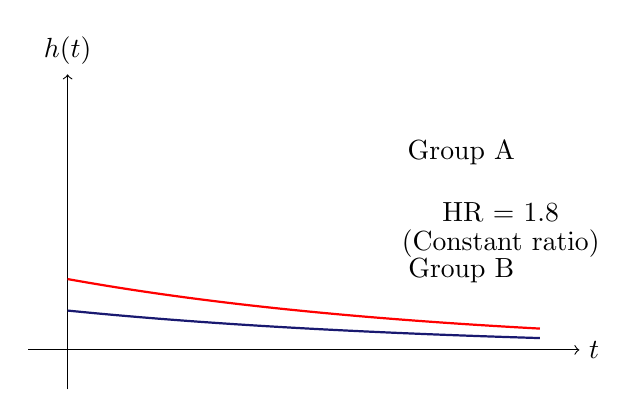
\begin{tikzpicture}[domain=0:6, smooth, samples=100]
\draw[->] (-0.5,0) -- (6.5,0) node[right] {$t$};
\draw[->] (0,-0.5) -- (0,3.5) node[above] {$h(t)$};

\draw[thick, MidnightBlue] plot (\x, {0.5*exp(-0.2*\x)});
\draw[thick, red] plot (\x, {0.5*exp(-0.2*\x)*1.8});

\node at (5,2.5) {Group A};
\node at (5,1) {Group B};
\node at (5.5,1.75) {HR = 1.8};
\node at (5.5,1.35) {(Constant ratio)};
\end{tikzpicture}
\end{frame}

\subsection{Hazard Ratios: Definition and Interpretation}

\begin{frame}{The Hazard Ratio as a Measure of Effect}
The hazard ratio (HR) is the primary measure of association in survival analysis:

\begin{definition}[Hazard Ratio]
The hazard ratio compares the hazards of two groups:
$$\text{HR} = \frac{h(t|X_A)}{h(t|X_B)} = \exp\left(\beta^T (X_A - X_B)\right)$$
The baseline hazard cancels out, leaving only the covariate effects.
\end{definition}

\begin{block}{Key Result}
$$\text{HR} = \exp(\beta_j)$$
The exponentiated coefficient directly gives the hazard ratio for a one-unit change.
\end{block}
\end{frame}

\begin{frame}{Interpretation of Hazard Ratios}
\tikzstyle{interpretation} = [rectangle, rounded corners, minimum width=10cm, minimum height=0.9cm, text centered]

\begin{tikzpicture}[node distance=1.2cm]
\node (I1) [interpretation, draw=Green, fill=green!10] {$\\beta > 0 \\implies \\text{HR} > 1$: The covariate increases the hazard (risk factor)};
\node (I2) [interpretation, below of=I1, draw=MidnightBlue, fill=blue!10] {$\\beta = 0 \\implies \\text{HR} = 1$: No association};
\node (I3) [interpretation, below of=I2, draw=Red, fill=red!10] {$\\beta < 0 \\implies \\text{HR} < 1$: The covariate decreases the hazard (protective factor)};
\end{tikzpicture}
\end{frame}

\begin{frame}{Numerical Interpretation Examples}
\begin{tabular}{cccc}
\toprule
$\beta$ & HR = $\exp(\beta)$ & Interpretation & 95\% CI for HR \\
\midrule
0 & 1.00 & No effect & (0.82, 1.22) \\
0.10 & 1.11 & 11\% increased hazard & (0.91, 1.35) \\
0.50 & 1.65 & 65\% increased hazard & (1.35, 2.02) \\
1.00 & 2.72 & 172\% increased hazard & (2.23, 3.32) \\
-0.50 & 0.61 & 39\% decreased hazard & (0.50, 0.74) \\
-1.00 & 0.37 & 63\% decreased hazard & (0.30, 0.45) \\
\bottomrule
\end{tabular}
\end{frame}

\begin{frame}{Continuous Covariates: Unit Changes}
For a continuous predictor, the HR represents the hazard ratio per unit increase:

\begin{block}{Example: Age and Cardiovascular Disease}
If $\beta_{\text{age}} = 0.08$ (per year):
\begin{itemize}
\item Per 1 year: $\text{HR} = \exp(0.08) = 1.083$ (8.3\% increased hazard)
\item Per 10 years: $\text{HR} = \exp(0.80) = 2.23$ (123\% increased hazard)
\end{itemize}
\end{block}
\end{frame}

\begin{frame}{Q2 Summary: Key Equations}
\begin{small}
\begin{align*}
\textbf{Hazard Function:} \quad & h(t) = \\lim_{\\Delta t \\to 0} \\frac{P(t \\le T < t + \\Delta t | T \\ge t)}{\\Delta t} \\\\
\textbf{Survival Function:} \quad & S(t) = P(T > t) \\\\
\textbf{Cox Model:} \quad & h(t|X) = h_0(t) \\exp(\\beta_1 X_1 + \\cdots + \\beta_k X_k) \\\\
\textbf{Hazard Ratio:} \quad & \\text{HR} = \\exp(\\beta_j) \\\\
\textbf{Data:} \quad & \\text{Observed time } t_i = \\min(T_i, C_i), \\quad \\delta_i = I(T_i \\le C_i)
\end{align*}
\end{small}
\end{frame}

% ============================================================================
% PART Q3: PRINCIPAL COMPONENT ANALYSIS
% ============================================================================

\section{Q3: Principal Component Analysis for Dimensionality Reduction}

\subsection{Foundational Concepts of PCA}

\begin{frame}{What is Principal Component Analysis?}
Principal Component Analysis (PCA) is a linear dimensionality reduction technique:

\begin{block}{Definition}
PCA is an unsupervised learning technique that transforms a set of correlated variables into a smaller set of uncorrelated variables called \textbf{principal components} (PCs), while retaining the maximum possible variance in the original data.
\end{block}

\tikzstyle{block} = [rectangle, rounded corners, minimum width=4cm, minimum height=1.5cm, text centered, draw=MidnightBlue, fill=blue!10]
\tikzstyle{arrow} = [thick,->,>=stealth]

\begin{tikzpicture}[node distance=2cm]
\node (input) [block] {Original Data\\$n \\times p$ matrix\\$p = 15$ indicators};
\node (pca) [block, right of=input, xshift=5cm] {PCA\\Transformation};
\node (output) [block, right of=pca, xshift=5cm] {Reduced Data\\$n \\times k$ matrix\\$k = 4$ components};

\draw [arrow] (input) -- (pca) node[midway, above] {Linear\\projection};
\draw [arrow] (pca) -- (output) node[midway, above] {Variance\\maximization};
\end{tikzpicture}
\end{frame}

\begin{frame}{Geometric Interpretation of PCA}
PCA finds the directions of maximum variance in the data:

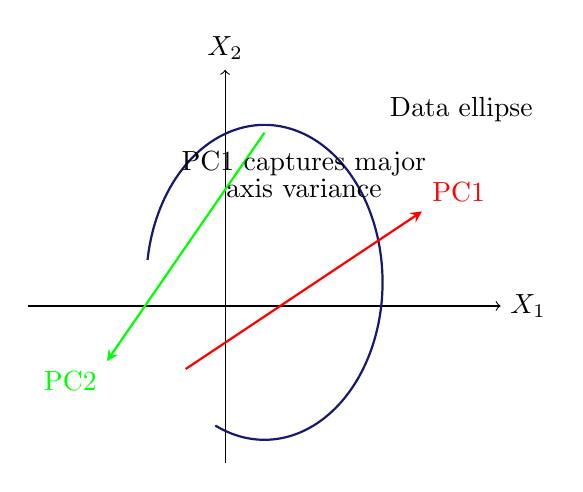
\begin{tikzpicture}[domain=-2:3, smooth, samples=100]
\draw[->] (-2.5,0) -- (3.5,0) node[right] {$X_1$};
\draw[->] (0,-2) -- (0,3) node[above] {$X_2$};

\draw[thick, MidnightBlue] plot ({1.5*cos(deg(\x)) + 0.5}, {2*sin(deg(\x)) + 0.3});

\draw[->, thick, red, >=stealth] (-0.5,-0.8) -- (2.5,1.2) node[above right] {PC1};
\draw[->, thick, green, >=stealth] (0.5,2.2) -- (-1.5,-0.7) node[below left] {PC2};

\node at (3,2.5) {Data ellipse};
\node at (1,1.8) {PC1 captures major};
\node at (1,1.5) {axis variance};
\end{tikzpicture}

\begin{block}{Key Principle}
PC1 captures the maximum variance direction; PC2 is orthogonal to PC1 and captures remaining maximum variance.
\end{block}
\end{frame}

\begin{frame}{Mathematical Formulation of PCA}
The goal of PCA is to find a linear transformation that maximizes variance:

\begin{block}{Data Matrix}
Let $\mathbf{X}$ be an $n \times p$ data matrix where:
\begin{itemize}
\item $n$: Number of observations (patients)
\item $p$: Number of variables (15 clinical indicators)
\end{itemize}
\end{block}

\begin{block}{Principal Components as Linear Combinations}
Each principal component $PC_j$ is a linear combination:
$$PC_j = a_{j1}X_1 + a_{j2}X_2 + \cdots + a_{jp}X_p$$
where $\mathbf{a}_j = (a_{j1}, \ldots, a_{jp})$ is the loading vector (eigenvector).
\end{block}
\end{frame}

\begin{frame}{The Problem of Dimensionality in Clinical Research}
Modern clinical studies often collect numerous measurements per patient:

\tikzstyle{challenge} = [rectangle, rounded corners, minimum width=10cm, minimum height=1cm, text centered]

\begin{tikzpicture}[node distance=1.5cm]
\node (C1) [challenge, draw=Red, fill=red!10] {High correlation among clinical indicators};
\node (C2) [challenge, below of=C1, draw=Orange, fill=orange!10] {Small sample sizes relative to number of variables};
\node (C3) [challenge, below of=C2, draw=Yellow, fill=yellow!10] {Multicollinearity complicates regression modeling};
\node (C4) [challenge, below of=C3, draw=MidnightBlue, fill=blue!10] {Difficult interpretation of 15+ correlated variables};
\end{tikzpicture}
\end{frame}

\begin{frame}{Benefits of Dimensionality Reduction}
Reducing 15 indicators to 4 principal components offers several advantages:

\tikzstyle{benefit} = [rectangle, rounded corners, minimum width=10cm, minimum height=0.9cm, text centered]

\begin{tikzpicture}[node distance=1.2cm]
\node (B1) [benefit, draw=MidnightBlue, fill=blue!10] {Dimensionality reduction: 15 $\\rightarrow$ 4 variables (73\% reduction)};
\node (B2) [benefit, below of=B1, draw=Green, fill=green!10] {Decorrelation: Components are uncorrelated (eliminates multicollinearity)};
\node (B3) [benefit, below of=B2, draw=Orange, fill=orange!10] {Noise reduction: Low-variance components often capture measurement error};
\node (B4) [benefit, below of=B3, draw=Purple, fill=purple!10] {Interpretability: Each PC represents a clinical dimension};
\end{tikzpicture}
\end{frame}

\begin{frame}{Step 1: Data Standardization}
Before performing PCA, variables must be standardized:

\begin{block}{Standardization Formula}
For each variable $X_j$:
$$Z_{ij} = \frac{X_{ij} - \bar{X}_j}{s_j}$$
where $\bar{X}_j$ is the mean and $s_j$ is the standard deviation.
\end{block}

\begin{block}{Problem of Scale Differences}
Clinical indicators often have different scales (e.g., BP in mmHg, cholesterol in mg/dL). Without standardization, larger-scale variables would dominate.
\end{block}

\begin{block}{Result}
After standardization, each variable has mean 0 and variance 1.
\end{block}
\end{frame}

\begin{frame}{Step 2: Computing the Covariance/Correlation Matrix}
The covariance matrix captures the relationships between variables:

\begin{block}{Sample Correlation Matrix}
For standardized data $\mathbf{Z}$:
$$\mathbf{R} = \frac{1}{n-1} \mathbf{Z}^T \mathbf{Z}$$
where $\mathbf{R}$ is a $p \times p$ symmetric matrix with 1s on the diagonal.
\end{block}

\begin{block}{Example Correlations in Clinical Data}
\begin{tabular}{llc}
\toprule
Variable Pair & Interpretation & Correlation \\
\midrule
Systolic BP - Diastolic BP & Strong positive & 0.78 \\
HDL - Triglycerides & Moderate negative & -0.52 \\
Creatinine - eGFR & Strong negative & -0.85 \\
\bottomrule
\end{tabular}
\end{block}
\end{frame}

\begin{frame}{Step 3: Eigenvalue Decomposition}
The core of PCA is the eigenvalue decomposition of the correlation matrix:

\begin{block}{Eigenvalue Equation}
Find eigenvalues $\lambda_j$ and eigenvectors $\mathbf{v}_j$ such that:
$$\mathbf{R} \mathbf{v}_j = \lambda_j \mathbf{v}_j$$
where $\mathbf{v}_j^T \mathbf{v}_j = 1$ and $\mathbf{v}_j^T \mathbf{v}_k = 0$ for $j \neq k$.
\end{block}

\begin{block}{Eigen Decomposition}
$$\mathbf{R} = \mathbf{V} \boldsymbol{\Lambda} \mathbf{V}^T$$
where $\mathbf{V}$ contains eigenvectors and $\boldsymbol{\Lambda} = \text{diag}(\lambda_1, \ldots, \lambda_p)$.
\end{block}

\begin{block}{Properties}
Eigenvalues $\lambda_j \geq 0$ (since $\mathbf{R}$ is positive semi-definite).
\end{block}
\end{frame}

\begin{frame}{Eigenvalues as Variance Explained}
Each eigenvalue represents the variance explained by its corresponding principal component:

\begin{block}{Variance Interpretation}
For standardized data: $\lambda_j = \text{Var}(PC_j)$ and $\sum_{j=1}^{p} \lambda_j = p$.
\end{block}

\begin{block}{Example Eigenvalue Spectrum}
\begin{tabular}{cccc}
\toprule
Component & Eigenvalue ($\lambda_j$) & Variance \% & Cumulative \% \\
\midrule
PC1 & 4.52 & 30.1 & 30.1 \\
PC2 & 2.87 & 19.1 & 49.2 \\
PC3 & 2.14 & 14.3 & 63.5 \\
PC4 & 1.68 & 11.2 & 74.7 \\
\bottomrule
\end{tabular}
\end{block}
\end{frame}

\begin{frame}{Step-by-Step Algorithm Summary}
\tikzstyle{step} = [rectangle, rounded corners, minimum width=12cm, minimum height=0.9cm, text centered]

\begin{tikzpicture}[node distance=1cm]
\node (S1) [step, draw=MidnightBlue, fill=blue!10] {\textbf{Step 1:} Standardize data: $Z_{ij} = (X_{ij} - \\bar{X}_j) / s_j$};
\node (S2) [step, below of=S1, draw=Green, fill=green!10] {\textbf{Step 2:} Compute correlation matrix: $\\mathbf{R} = \\frac{1}{n-1}\\mathbf{Z}^T\\mathbf{Z}$};
\node (S3) [step, below of=S2, draw=Orange, fill=orange!10] {\textbf{Step 3:} Eigenvalue decomposition: $\\mathbf{R}\\mathbf{v}_j = \\lambda_j\\mathbf{v}_j$};
\node (S4) [step, below of=S3, draw=Purple, fill=purple!10] {\textbf{Step 4:} Order by eigenvalues: $\\lambda_1 \\ge \\lambda_2 \\ge \\cdots \\ge \\lambda_{15}$};
\node (S5) [step, below of=S4, draw=Red, fill=red!10] {\textbf{Step 5:} Select top $k$ components and compute scores: $\\mathbf{PC} = \\mathbf{Z}\\mathbf{V}_k$};
\end{tikzpicture}
\end{frame}

\begin{frame}{Scree Plot for Component Selection}
The scree plot visualizes eigenvalues to guide component selection:

\begin{tikzpicture}[domain=0.5:15.5, samples=15]
\draw[->] (0,0) -- (16,0) node[right] {Component Number};
\draw[->] (0,0) -- (0,5) node[above] {Eigenvalue};

\draw[thick, MidnightBlue, mark=*, mark size=3pt] plot coordinates {
(1,4.52)
(2,2.87)
(3,2.14)
(4,1.68)
(5,1.23)
(6,0.95)
(7,0.72)
(8,0.58)
(9,0.45)
(10,0.35)
(11,0.28)
(12,0.24)
(13,0.21)
(14,0.18)
(15,0.15)
};

\draw[dashed, red] (0,1) -- (16,1) node[right at={(16,1)}] {Kaiser criterion ($\\lambda=1$)};

\node[circle, draw=Red, fill=red!10, minimum size=0.3cm] at (4,1.68) {};

\node at (10,4) {Scree Plot};
\node at (10,3.5) {Elbow at PC4};
\end{tikzpicture}
\end{frame}

\begin{frame}{Justifying 4 Principal Components}
Several criteria support selecting 4 components from 15:

\begin{block}{Kaiser Criterion}
Retain components with eigenvalue > 1:
PC1 ($\lambda=4.52$), PC2 ($\lambda=2.87$), PC3 ($\lambda=2.14$), PC4 ($\lambda=1.68$) all exceed 1.
\end{block}

\begin{block}{Cumulative Variance}
4 components explain 74.7\% of total variance, exceeding the commonly recommended 70-75\% threshold.
\end{block}

\begin{block}{Elbow Criterion}
Visual inspection of the scree plot shows an elbow at PC4.
\end{block}
\end{frame}

\begin{frame}{Interpreting Principal Components in Clinical Context}
Each principal component represents a clinical dimension:

\begin{tabular}{lp{8cm}c}
\toprule
Component & Clinical Interpretation & Variance \% \\
\midrule
PC1 & \textbf{Cardiovascular Risk}: Systolic BP, Diastolic BP, Pulse Pressure, LDL, Triglycerides & 30.1 \\
\midrule
PC2 & \textbf{Metabolic Syndrome}: BMI, Waist Circumference, Fasting Glucose, HbA1c & 19.1 \\
\midrule
PC3 & \textbf{Inflammatory Status}: CRP, ESR, WBC Count & 14.3 \\
\midrule
PC4 & \textbf{Renal Function}: Creatinine, eGFR & 11.2 \\
\bottomrule
\end{tabular}

Cumulative variance: 74.7\% retained.
\end{frame}

\begin{frame}{Computing Principal Component Scores}
Principal component scores are used for subsequent analysis:

\begin{block}{Score Calculation}
For each observation $i$ and component $j$:
$$PC_{ij} = z_{i1}v_{1j} + z_{i2}v_{2j} + \cdots + z_{i,15}v_{15,j}$$
In matrix form: $\mathbf{PC} = \mathbf{Z}\mathbf{V}_4$
\end{block}

\begin{block}{Properties of Scores}
\begin{itemize}
\item Each column has mean 0
\item Each column has variance equal to the corresponding eigenvalue
\end{itemize}
\end{block}
\end{frame}

\begin{frame}{Biplot for Joint Interpretation}
The biplot visualizes observations and variables simultaneously:

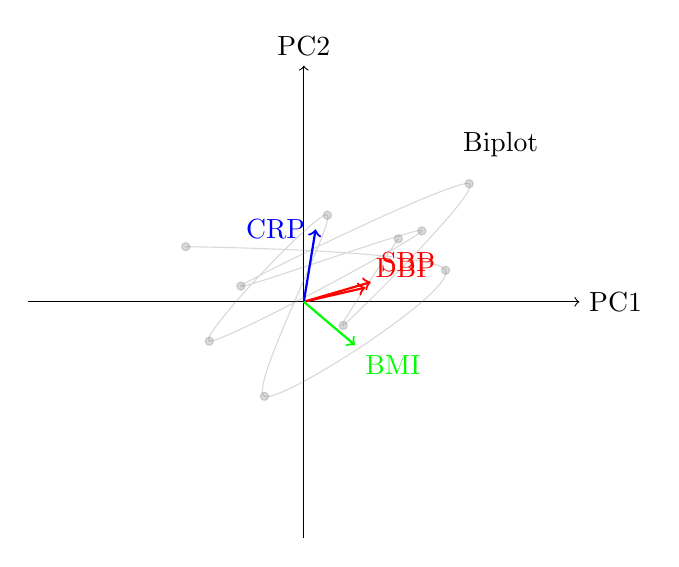
\begin{tikzpicture}[domain=-3:3, smooth, samples=50]
\draw[->] (-3.5,0) -- (3.5,0) node[right] {PC1};
\draw[->] (0,-3) -- (0,3) node[above] {PC2};

\draw[gray, opacity=0.3, mark=*, mark size=1.5pt] plot coordinates {
(1.2,0.8) (0.5,-0.3) (2.1,1.5) (-0.8,0.2) (1.5,0.9)
(-1.2,-0.5) (0.3,1.1) (-0.5,-1.2) (1.8,0.4) (-1.5,0.7)
};

\draw[->, thick, red] (0,0) -- (0.85,0.25) node[above right] {SBP};
\draw[->, thick, red] (0,0) -- (0.78,0.18) node[above right] {DBP};
\draw[->, thick, blue] (0,0) -- (0.15,0.92) node[left] {CRP};
\draw[->, thick, green] (0,0) -- (0.65,-0.55) node[below right] {BMI};

\node at (2.5,2) {Biplot};
\end{tikzpicture}

\begin{block}{Biplot Interpretation}
Points = patient scores; Arrows = variable loadings.
\end{block}
\end{frame}

\begin{frame}{Limitations of PCA}
PCA has important limitations:

\tikzstyle{limitation} = [rectangle, rounded corners, minimum width=11cm, minimum height=0.9cm, text centered]

\begin{tikzpicture}[node distance=1cm]
\node (L1) [limitation, draw=Red, fill=red!10] {\textbf{Linearity}: PCA only captures linear relationships};
\node (L2) [limitation, below of=L1, draw=Orange, fill=orange!10] {\textbf{No class discrimination}: Components may not separate disease groups};
\node (L3) [limitation, below of=L2, draw=Yellow, fill=yellow!10] {\textbf{Interpretability}: Component meaning may be unclear};
\node (L4) [limitation, below of=L3, draw=MidnightBlue, fill=blue!10] {\textbf{Information loss}: Some variance is discarded};
\end{tikzpicture}
\end{frame}

\begin{frame}{Q3 Summary: Key Equations}
\begin{small}
\begin{align*}
\textbf{Standardization:} \quad & Z_{ij} = \\frac{X_{ij} - \\bar{X}_j}{s_j} \\\\
\textbf{Correlation Matrix:} \quad & \\mathbf{R} = \\frac{1}{n-1}\\mathbf{Z}^T\\mathbf{Z} \\\\
\textbf{Eigen Decomposition:} \quad & \\mathbf{R}\\mathbf{v}_j = \\lambda_j\\mathbf{v}_j \\\\
\textbf{Variance Explained:} \quad & \\text{VE}_j = \\frac{\\lambda_j}{\\sum_{m=1}^{15}\\lambda_m} \\times 100\\% \\\\
\textbf{Component Scores:} \quad & PC_{ij} = \\sum_{k=1}^{15} z_{ik}v_{kj} \\\\
\textbf{Cumulative Variance:} \quad & \\text{CVE}_4 = 74.7\\%
\end{align*}
\end{small}
\end{frame}

% ============================================================================
% PART Q4: MACHINE LEARNING WORKFLOW IN HOSPITAL SETTINGS
% ============================================================================

\section{Q4: Machine Learning Workflow in a Hospital Setting}

\subsection{Purpose of ML in Healthcare}

\begin{frame}{Why Machine Learning in Healthcare?}
Machine learning represents a transformative paradigm in healthcare delivery:

\begin{itemize}
\item \textbf{Clinical Decision Support}: Real-time risk stratification and early warning systems for sepsis, cardiac arrest, and deterioration.
\item \textbf{Operational Efficiency}: Resource allocation optimization, patient flow management, and predictive scheduling.
\item \textbf{Diagnostic Accuracy}: Enhanced image interpretation, pattern recognition in laboratory data, and differential diagnosis assistance.
\item \textbf{Predictive Analytics}: Hospital readmission prediction, length of stay estimation, and population health management.
\end{itemize}

The fundamental shift involves moving from reactive medicine to proactive, personalized, and precision-based clinical interventions.
\end{frame}

\begin{frame}{From Retrospective Analysis to Real-Time Clinical Applications}
Machine learning enables a paradigm shift toward real-time predictions:

\begin{itemize}
\item \textbf{Retrospective Phase}: Secondary analysis of administrative claims, quality improvement initiatives.
\item \textbf{Proactive Phase}: Prospective risk modeling embedded within electronic health record systems.
\item \textbf{Real-Time Phase}: Streaming analytics providing continuous risk scores and actionable alerts at the point of care.
\end{itemize}

\begin{block}{Key Distinction}
The transition from descriptive and diagnostic analytics to predictive and prescriptive analytics represents the core value proposition of ML in modern hospital settings.
\end{block}
\end{frame}

\begin{frame}{Defining the Clinical Problem}
The foundation of any successful ML implementation begins with a precisely formulated clinical question:

\begin{itemize}
\item \textbf{Clinical Validity}: Does the outcome have clinical significance and actionable intervention options?
\item \textbf{Feasibility Assessment}: Are the required data elements available and of sufficient quality?
\item \textbf{Stakeholder Alignment}: Engagement with clinical champions, informaticists, and administrative leadership.
\item \textbf{Success Metrics}: Clear definition of primary and secondary outcomes.
\end{itemize}

Common applications include mortality prediction, readmission risk, sepsis early warning, and length of stay estimation.
\end{frame}

\begin{frame}{Data Sources in Hospital Settings}
Hospital data ecosystems comprise multiple interconnected sources:

\begin{itemize}
\item \textbf{Electronic Health Records (EHR)}: Demographics, vital signs, laboratory results, medications, procedures, clinical notes.
\item \textbf{Administrative Data}: Billing codes, diagnosis codes (ICD-10), procedure codes (CPT), discharge summaries.
\item \textbf{Real-Time Monitoring Data}: Bedside monitors, infusion pumps, ventilators, and other connected medical devices.
\item \textbf{External Data Sources}: Social determinants of health, regional epidemiological data.
\end{itemize}

\begin{block}{Interoperability Standards}
HL7 FHIR (Fast Healthcare Interoperability Resources) serves as the primary standard for healthcare data exchange.
\end{block}
\end{frame}

\begin{frame}{Data Quality and Preprocessing Challenges}
Healthcare data presents unique preprocessing challenges:

\begin{itemize}
\item \textbf{Missing Data}: Systematic patterns of missingness (MNAR, MAR, MCAR) require appropriate imputation strategies.
\item \textbf{Temporal Heterogeneity}: Changes in clinical practices over time introduce distribution shifts.
\item \textbf{Irregular Sampling}: Laboratory results and vital signs at irregular intervals.
\item \textbf{Coding Variations}: ICD-10 code granularity and evolving code sets require standardization.
\end{itemize}
\end{frame}

\begin{frame}{Feature Engineering in Clinical Domains}
Feature engineering transforms raw clinical data into meaningful predictors:

\begin{itemize}
\item \textbf{Temporal Aggregation}: Computing trends, rates of change (e.g., delta neutrophil index, shock index).
\item \textbf{Domain-Specific Transformations}: Composite scores such as SOFA, NEWS, and qSOFA.
\item \textbf{Natural Language Processing}: Extraction of clinical entities from unstructured notes.
\item \textbf{Categorical Encodings}: Hierarchical groupings of diagnoses and procedures.
\end{itemize}
\end{frame}

\begin{frame}{Feature Selection Strategies}
Feature selection aims to identify the most predictive subset of features:

\begin{itemize}
\item \textbf{Filter Methods}: Correlation analysis, mutual information, variance thresholds.
\item \textbf{Wrapper Methods}: Recursive feature elimination (RFE), forward/backward selection.
\item \textbf{Embedded Methods}: L1 regularization (LASSO), tree-based importance scores.
\item \textbf{Clinical Validation}: Feature review by subject matter experts.
\end{itemize}

Balancing statistical significance with clinical interpretability is crucial.
\end{frame}

\begin{frame}{Model Selection Considerations}
The selection of ML algorithms requires careful consideration of trade-offs:

\begin{itemize}
\item \textbf{Interpretable Models}: Logistic regression, decision trees, score-based models.
\item \textbf{Black-Box Models}: Gradient boosting machines, random forests, deep neural networks.
\item \textbf{Time-to-Event Models}: Cox proportional hazards for survival outcomes.
\end{itemize}

\begin{block}{The Interpretability-Performance Trade-off}
While complex models may achieve higher discrimination, interpretable models facilitate clinical acceptance and regulatory review.
\end{block}
\end{frame}

\begin{frame}{Model Training Best Practices}
Rigorous model training protocols ensure reproducibility and generalizability:

\begin{itemize}
\item \textbf{Train-Validation-Test Split}: Temporal splits for time-series data to prevent data leakage.
\item \textbf{Cross-Validation}: Stratified k-fold cross-validation for robust performance estimation.
\item \textbf{Class Imbalance Handling}: SMOTE, class weighting, threshold optimization.
\item \textbf{Hyperparameter Tuning}: Grid search, random search, or Bayesian optimization.
\end{itemize}
\end{frame}

\begin{frame}{Validation Strategies}
Comprehensive validation assesses performance across multiple dimensions:

\begin{itemize}
\item \textbf{Internal Validation}: Bootstrap and cross-validation estimates.
\item \textbf{Temporal Validation}: Performance on holdout data from a later time period.
\item \textbf{External Validation}: Testing on independent datasets from different institutions.
\item \textbf{Subgroup Validation}: Performance assessment across demographic subgroups.
\end{itemize}
\end{frame}

\begin{frame}{Performance Metrics for Clinical Models}
Evaluation metrics must align with clinical objectives:

\begin{itemize}
\item \textbf{Discrimination}: Area under the ROC curve (AUC-ROC).
\item \textbf{Calibration}: Hosmer-Lemeshow test, calibration curves, Brier score.
\item \textbf{Clinical Utility}: Decision curve analysis and net benefit calculations.
\item \textbf{Sensitivity and Specificity}: Performance at clinically relevant operating points.
\end{itemize}
\end{frame}

\begin{frame}{Deployment Strategies}
Transitioning from research prototypes to clinical systems:

\begin{itemize}
\item \textbf{Shadow Mode Deployment}: Running the model without exposing predictions to end-users.
\item \textbf{Pilot Implementation}: Limited deployment in specific clinical units with enhanced monitoring.
\item \textbf{Full Integration}: Production deployment within the EHR with user-facing interfaces.
\end{itemize}

Technical infrastructure must support real-time inference and high availability.
\end{frame}

\begin{frame}{Integration into Clinical Workflows}
Successful deployment depends on thoughtful integration:

\begin{itemize}
\item \textbf{User Interface Design}: In-context displays within clinician workflows.
\item \textbf{Alert Design}: Tiered alert severity, clear explanatory information.
\item \textbf{Feedback Mechanisms}: Capture of clinician acceptance/rejection for improvement.
\item \textbf{EHR Integration Standards}: SMART on FHIR applications for interoperability.
\end{itemize}
\end{frame}

\begin{frame}{Model Governance Framework}
Establishing robust governance structures ensures accountability:

\begin{itemize}
\item \textbf{Model Registry}: Documentation of model versions, training data, performance metrics.
\item \textbf{Approval Workflows}: Multidisciplinary review committees.
\item \textbf{Audit Trails}: Comprehensive logging of predictions and outcomes.
\item \textbf{Incident Response}: Defined procedures for model-related adverse events.
\end{itemize}
\end{frame}

\begin{frame}{Model Monitoring and Drift Detection}
Continuous monitoring is essential to detect performance degradation:

\begin{itemize}
\item \textbf{Data Drift Detection}: Statistical monitoring of input feature distributions.
\item \textbf{Concept Drift Detection}: Tracking of outcome rates over time.
\item \textbf{Performance Monitoring}: Ongoing calculation of performance metrics.
\item \textbf{Alert Thresholding}: Statistical process control methods.
\end{itemize}
\end{frame}

\begin{frame}{Model Updating and Retraining Strategies}
Maintaining model relevance requires planned updating protocols:

\begin{itemize}
\item \textbf{Scheduled Retraining}: Periodic updates based on accumulated new data.
\item \textbf{Triggered Retraining}: Updates initiated by detected performance degradation.
\item \textbf{Online Learning}: Continuous model adaptation with safeguards.
\item \textbf{Version Control}: Careful management of model versions with validation requirements.
\end{itemize}
\end{frame}

\begin{frame}{Data Privacy Requirements}
Healthcare ML development must comply with stringent privacy regulations:

\begin{itemize}
\item \textbf{Regulatory Compliance}: Adherence to HIPAA (US), GDPR (Europe).
\item \textbf{De-identification}: Safe harbor or expert determination methods.
\item \textbf{Access Controls}: Role-based access, audit logging, principle of least privilege.
\item \textbf{Consent Considerations}: Patient notification requirements for secondary data use.
\end{itemize}
\end{frame}

\begin{frame}{Ethical Considerations in Clinical ML}
Responsible development requires proactive attention to fairness:

\begin{itemize}
\item \textbf{Algorithmic Fairness}: Assessment of model performance across demographic groups.
\item \textbf{Bias Detection}: Analysis of training data for historical biases.
\item \textbf{Transparency}: Explainability features and clear communication about limitations.
\item \textbf{Accountability}: Clear lines of responsibility for model-related decisions.
\end{itemize}
\end{frame}

\begin{frame}{Regulatory Framework for Clinical AI}
Clinical ML systems may be subject to regulatory oversight:

\begin{itemize}
\item \textbf{SaMD Classification}: Software as a Medical Device framework from FDA, EU MDR.
\item \textbf{Risk-Based Validation}: Validation requirements scaled to risk level.
\item \textbf{Quality Management Systems}: FDA 21 CFR Part 820, ISO 13485.
\item \textbf{Post-Market Surveillance}: Ongoing monitoring and adverse event reporting.
\end{itemize}
\end{frame}

\begin{frame}{Example 1: Sepsis Early Warning System}
Sepsis prediction demonstrates the full workflow from problem definition to deployment:

\begin{itemize}
\item \textbf{Problem}: Early identification of patients at risk for timely antibiotic administration.
\item \textbf{Data}: Vital signs, laboratory values (lactate, WBC, creatinine), clinical notes.
\item \textbf{Features}: SOFA score components, infection indicators, temporal trends.
\item \textbf{Model}: Gradient boosting classifier with interpretability enhancements.
\item \textbf{Deployment}: Integrated into nursing station dashboards with tiered alerts.
\end{itemize}

Clinical studies have demonstrated reduced mortality with well-designed systems.
\end{frame}

\begin{frame}{Example 2: Radiology Image Triage}
Computer vision applications in radiology demonstrate ML potential:

\begin{itemize}
\item \textbf{Problem}: Prioritization of chest radiographs with acute findings (pneumothorax, pneumonia).
\item \textbf{Data}: Historical chest radiographs with radiologist annotations.
\item \textbf{Model}: Convolutional neural networks (CNN) for image classification.
\item \textbf{Deployment}: Integration with PACS systems to flag studies for expedited review.
\end{itemize}

These systems augment radiologist workflows without replacing human interpretation.
\end{frame}

\begin{frame}{Q4 Summary: Key Takeaways}
Successful implementation of ML in hospital settings requires attention to technical, organizational, and ethical dimensions:

\begin{itemize}
\item \textbf{Clinical Alignment}: ML solutions must address genuine clinical needs with actionable predictions.
\item \textbf{Data Foundation}: Robust data quality and preprocessing are prerequisites.
\item \textbf{Validation Rigor}: Comprehensive validation across temporal, external, and subgroup dimensions.
\item \textbf{Human-in-the-Loop}: Clinical ML should augment rather than replace human judgment.
\end{itemize}

\begin{block}{Final Message}
Machine learning holds tremendous promise for improving healthcare outcomes, but realizing this potential requires responsible development, rigorous validation, and sustained commitment to patient safety and ethical principles.
\end{block}
\end{frame}

% ============================================================================
% REFERENCES AND ACKNOWLEDGMENTS
% ============================================================================

\section{References}

\begin{frame}{References: Q1 - MLE and Logistic Regression}
\begin{small}
\begin{itemize}
\item Hosmer, D.W., Lemeshow, S., \& Sturdivant, R.X. (2013). Applied Logistic Regression (3rd ed.). Wiley.
\item Agresti, A. (2018). An Introduction to Categorical Data Analysis (3rd ed.). Wiley.
\item McCullagh, P. \& Nelder, J.A. (1989). Generalized Linear Models (2nd ed.). Chapman \& Hall.
\item Rothman, K.J., Greenland, S., \& Lash, T.L. (2008). Modern Epidemiology (3rd ed.). Lippincott Williams \& Wilkins.
\end{itemize}
\end{small}
\end{frame}

\begin{frame}{References: Q2 - Cox Proportional Hazards Model}
\begin{small}
\begin{itemize}
\item Cox, D.R. (1972). Regression Models and Life-Tables (with discussion). Journal of the Royal Statistical Society, Series B, 34(2), 187-220.
\item Kleinbaum, D.G. and Klein, M. (2012). Survival Analysis: A Self-Learning Text (3rd ed.). Springer.
\item Therneau, T.M. and Grambsch, P.M. (2000). Modeling Survival Data: Extending the Cox Model. Springer.
\item Hosmer, D.W., Lemeshow, S., and May, S. (2008). Applied Survival Analysis: Regression Modeling of Time to Event Data (2nd ed.). Wiley.
\end{itemize}
\end{small}
\end{frame}

\begin{frame}{References: Q3 - PCA and Q4 - ML Workflow}
\begin{small}
\begin{itemize}
\item Jolliffe, I.T. and Cadima, J. (2016). Principal component analysis: A review and recent developments. Philosophical Transactions of the Royal Society A, 374(2065), 20150202.
\item Ringnér, M. (2008). What is principal component analysis? Nature Biotechnology, 26(3), 303-304.
\item Hastie, T., Tibshirani, R., and Friedman, J. (2009). The Elements of Statistical Learning (2nd ed.). Springer.
\item Rajkomar, A., Oren, E., Chen, K., et al. (2018). Scalable and accurate deep learning with electronic health records. NPJ Digital Medicine, 1(1), 18.
\item FDA. (2019). Software as a Medical Device (SaMD): Clinical Evaluation. FDA Guidance Document.
\end{itemize}
\end{small}
\end{frame}

\begin{frame}{Course Information}
\begin{tabular}{ll}
\toprule
\textbf{Course} & \textbf{SDS6210 – Informatics for Health} \\
\midrule
Programme & MSc Public Health Data Science \\
Institution & Department of Public Health \\
Group & 5 \\
\midrule
Students: & Cavin Otieno (SDS6/46982/2024) \\
& Laura Nabalayo Kundu (SDS6/47543/2024) \\
& John Andrew (SDS6/47659/2024) \\
\bottomrule
\end{tabular}
\end{frame}

\end{document}
